\chapter{Progettazione Concettuale}

\section{Diagramma Delle Classi UML}

\begin{figure}[!h]
    \centering
    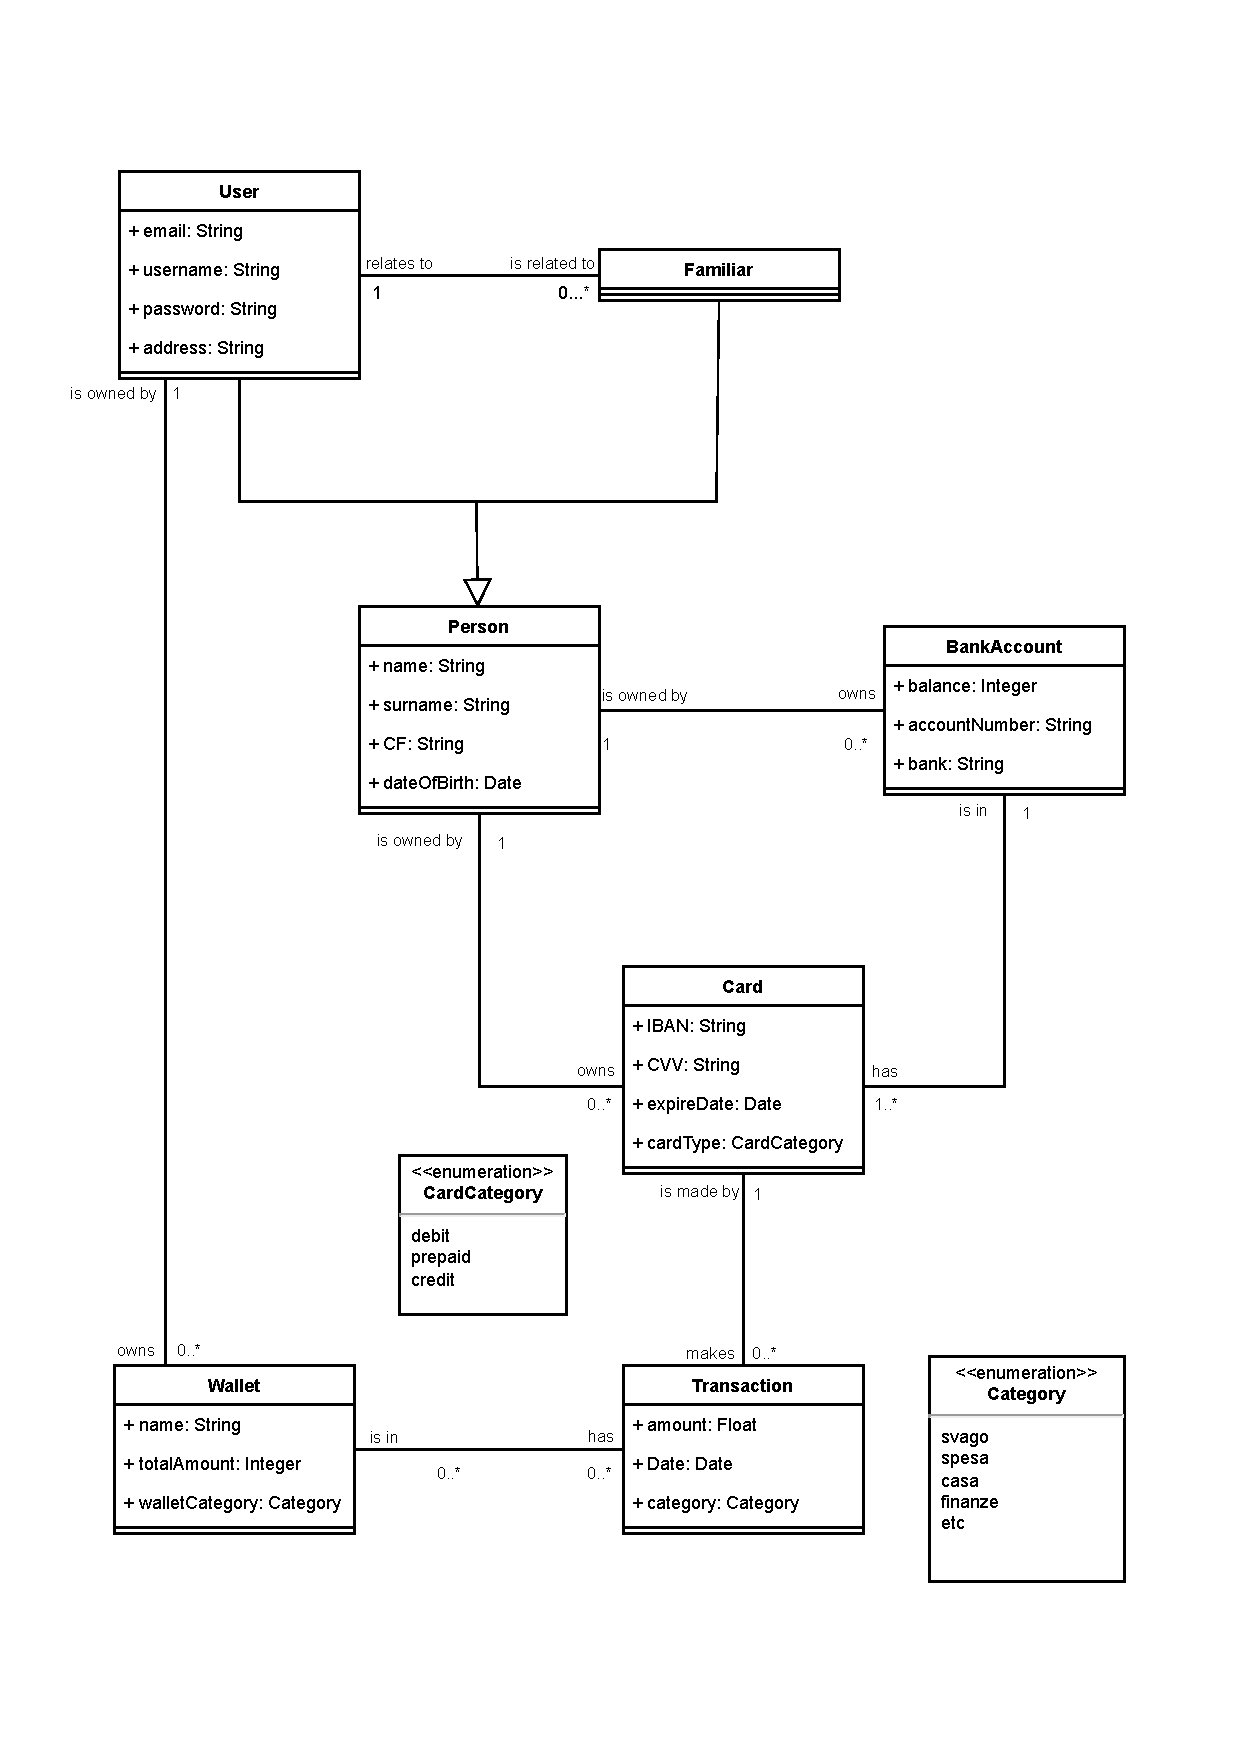
\includegraphics[scale=0.55]{pdfs/UMLdiagram.drawio.pdf}
    \caption{Diagramma UML}\label{UML}
\end{figure}

\section{Diagramma ER (Entità Relazione)}

\begin{figure}[!h]
    \centering
    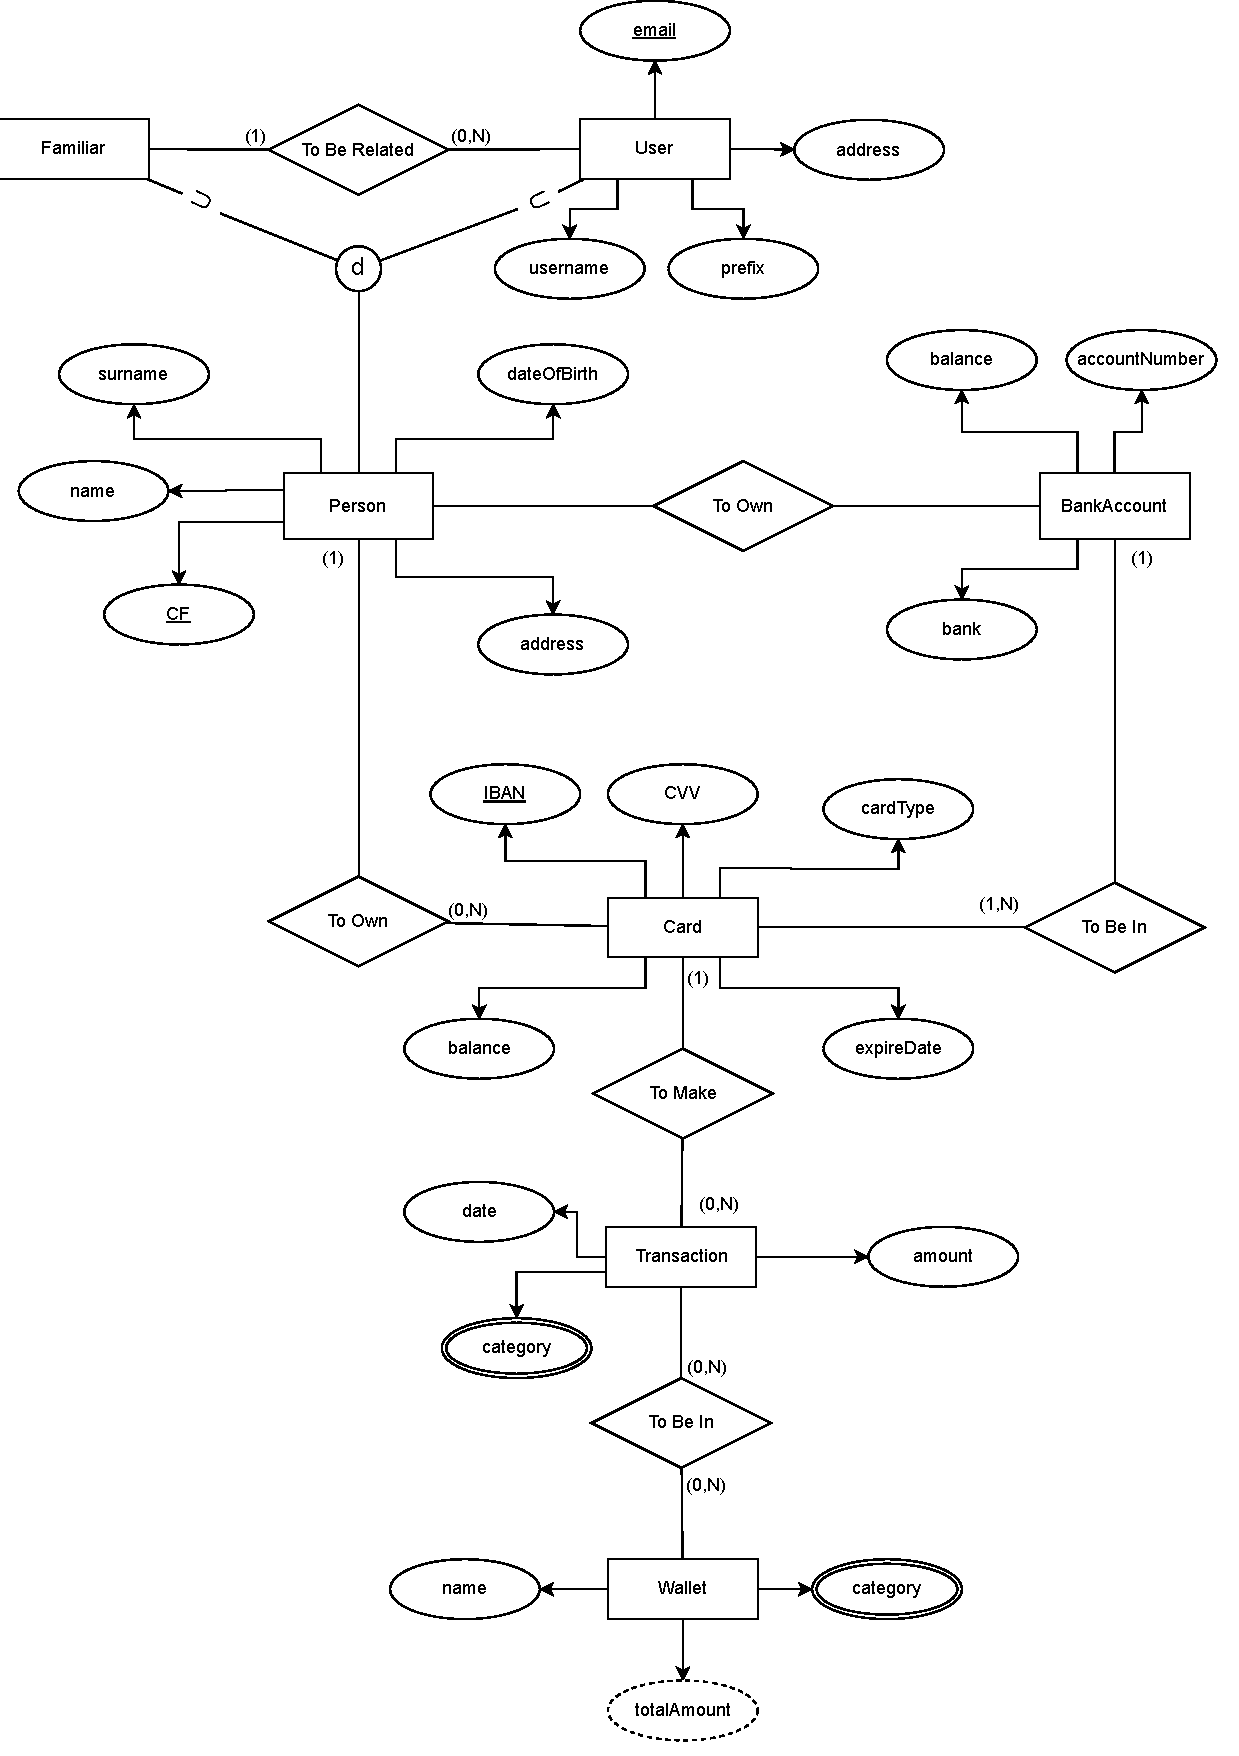
\includegraphics[scale=0.7]{pdfs/ERdiagram.drawio.pdf}
    \caption{Diagramma ER}\label{ER}
\end{figure}

\newpage

\section{Ristrutturazione}

\subsection{Attributi multipli}

Per quanto riguarda la gestione di attributi multipli,
abbiamo deciso di gestire l'attributo \textit{category} della tabella
\textbf{Transaction}, originariamente definito come enumerazione,
trasformandolo in una stringa, poiché non abbiamo bisogno di valori
specifici, trattandosi di una categoria personalizzabile.

Invece, per l'attributo \textit{cardType} della tabella \textbf{Card},
è stato deciso di non applicare lo stesso metodo, poiché le tipologie
di carte sono ben definite e non possono essere modificate.

\subsection{Generalizzazioni}

Per la generalizzazione, essendo di tipologia totale e disgiunta,
abbiamo optato per il metodo di eliminare la classe generale.
Abbiamo trasferito tutti gli attributi di essa nelle
classi specializzate, conservando le relative relazioni.

\subsection{Analisi degli identificativi}

Per la maggior parte delle classi, saranno utilizzati come identificativi
attributi già presenti di natura nelle classi stesse, poiché risultano
sufficienti e non richiedono l'uso di una chiave surrogata.
Tuttavia, in alcune classi, sono presenti chiavi surrogate,
identificate con il prefisso \textbf{ID\_}.

\newpage
\subsection{Diagramma UML ristrutturato}

\begin{figure}[!h]
    \centering
    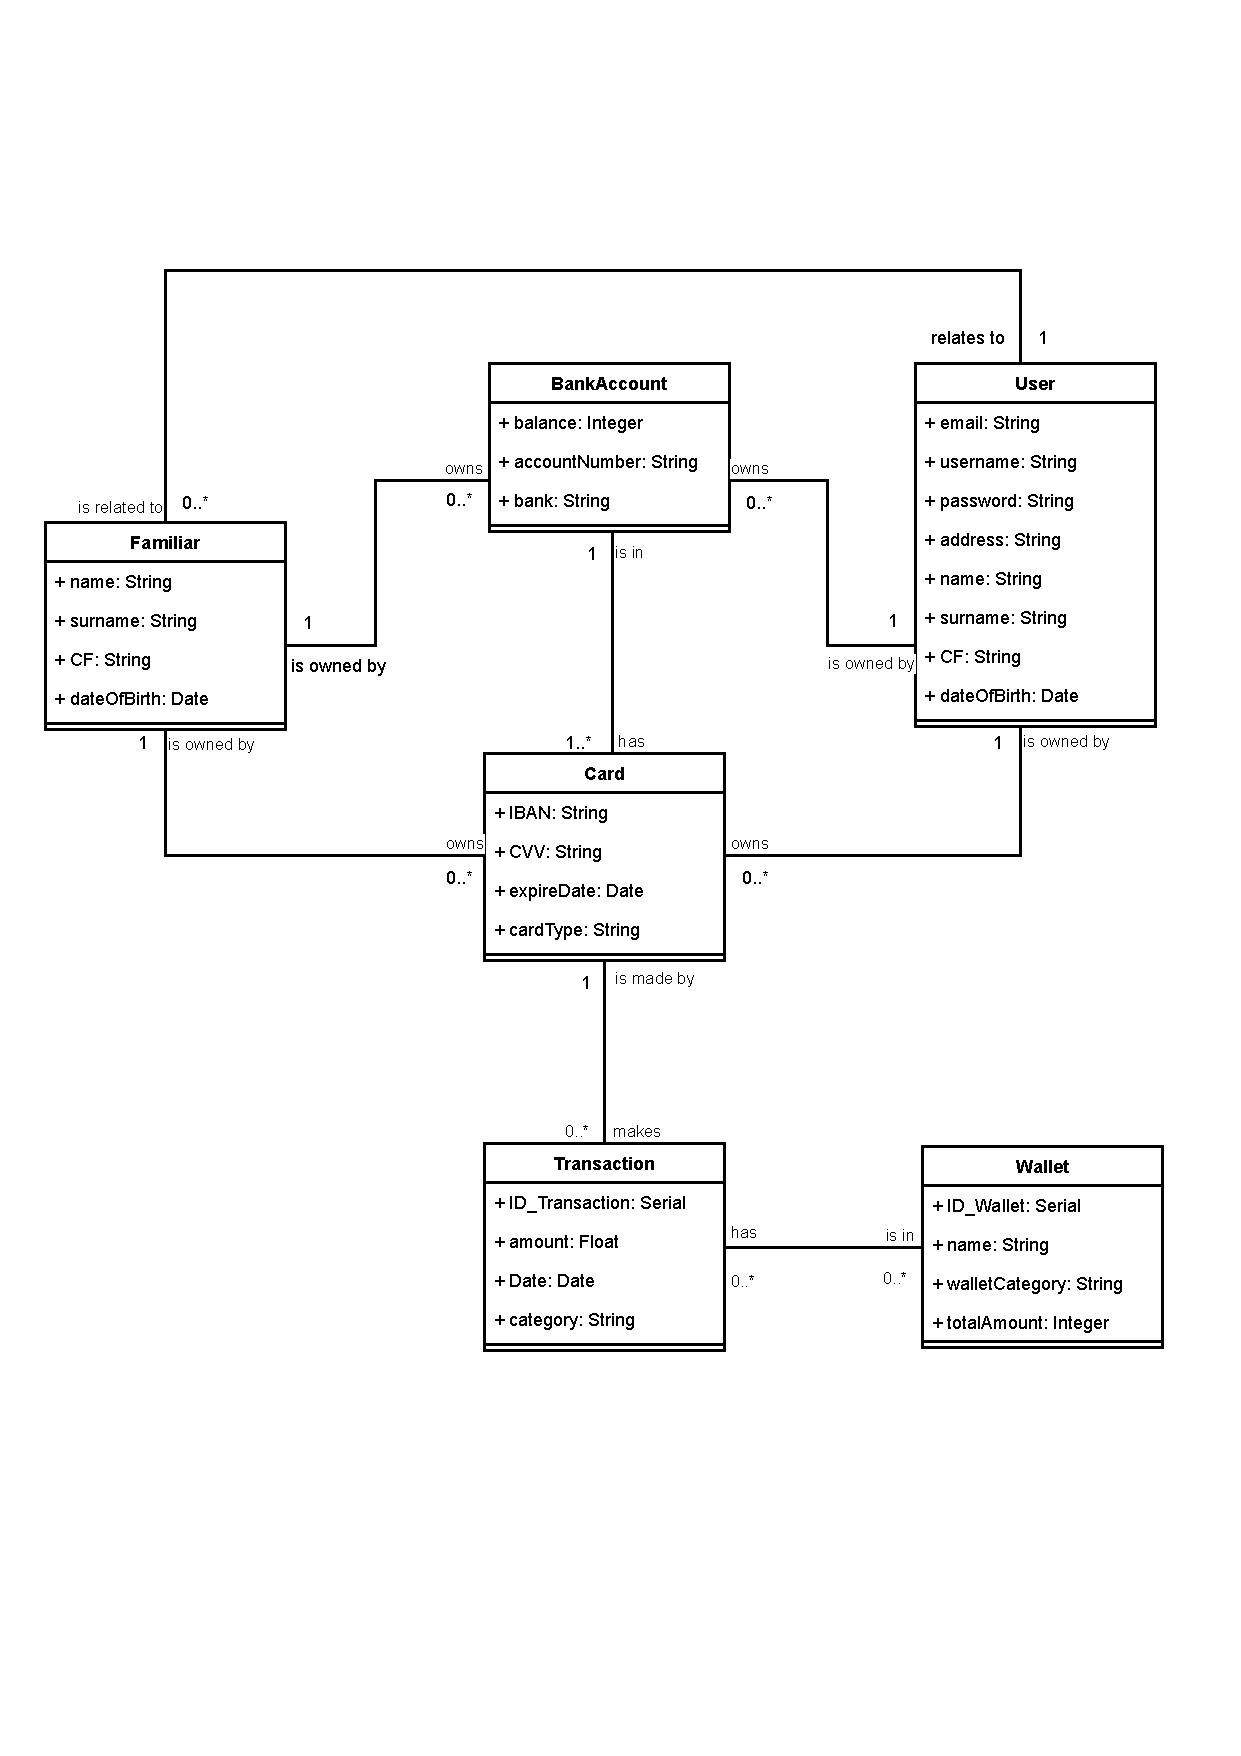
\includegraphics[scale=0.7]{pdfs/RestructuredUMLdiagram.drawio.pdf}
    \caption{Diagramma UML Ristrutturato}\label{ResUML}
\end{figure}

\newpage
\section{Dizionari}

\subsection{Dizionario delle classi}

\begin{longtable}{m{2.7cm}|m{4cm}|m{7cm}}

    \rowcolor{black!10}
    \textbf{Classe} & \textbf{Descrizione} & \textbf{Attributi} \\ \hline
    \endhead

    \textbf{User} & \raggedright Classe utilizzata per identificare gli utenti registrati alla piattaforma. &
    \parbox{7cm}{
        \textbf{email} (\textit{String}): email con la quale l'utente si è registrato. \\ 
        \textbf{username} (\textit{String}): chiave primaria, identificativa dell'utente. È anche il nome che viene mostrato per riconoscere lo stesso. \\
        \textbf{password} (\textit{String}): stringa atta alla convalidazione durante l'accesso all'account. \\
        \textbf{address} (\textit{String}): indirizzo del domicilio. \\
        \textbf{name} (\textit{String}): nome. \\
        \textbf{surname} (\textit{String}): cognome. \\
        \textbf{CF} (\textit{String}): codice fiscale. \\
        \textbf{dateOfBirth} (\textit{Date}): data di nascita.
    } \\ \hline

    \textbf{Familiar} & \raggedright Classe utilizzata per identificare i familiari degli utenti presenti nel database. &
    \parbox{7cm}{
        \textbf{name} (\textit{String}): nome. \\
        \textbf{surname} (\textit{String}): cognome. \\
        \textbf{CF} (\textit{String}): codice fiscale, chiave primaria nel caso del familiare. \\
        \textbf{dateOfBirth} (\textit{Date}): data di nascita.
    } \\ \hline

    \textbf{BankAccount} & \raggedright Classe utilizzata per identificare i conti correnti appartenenti a utenti o familiari. &
    \parbox{7cm}{
        \textbf{balance} (\textit{Integer}): indica il saldo disponibile sul conto corrente. \\
        \textbf{accountNumber} (\textit{String}): chiave primaria, identificativa del conto corrente. \\
        \textbf{bank} (\textit{String}): nome della banca alla quale è associato il conto corrente.
    } \\ \hline

    \textbf{Card} & \raggedright Classe utilizzata per identificare le carte appartenenti a utenti o familiari. &
    \parbox{7cm}{
        \textbf{IBAN} (\textit{String}): codice identificativo della carta. \\
        \textbf{CVV} (\textit{String}): codice di sicurezza per le transazioni delle carte. \\
        \textbf{expireDate} (\textit{Date}): data che indica la scadenza della carta. \\
        \textbf{cardType} (\textit{CardCategory}): campo che indica la tipologia della carta.
    } \\ \hline

    \textbf{Transaction} & \raggedright Classe utilizzata per tenere traccia di tutte le transazioni effettuate. &
    \parbox{7cm}{
        \textbf{ID\_Transaction} (\textit{Serial}): chiave surrogata, identificativo della singola transazione. \\
        \textbf{amount} (\textit{Float}): indica l'ammontare della transazione. \\
        \textbf{date} (\textit{Date}): data in cui è avvenuta la transazione. \\
        \textbf{category} (\textit{String}): tipologia di transazione. Serve per l'associazione automatica ai portafogli.
    } \\ \hline

    \textbf{Wallet} & \raggedright Classe utilizzata per raggruppare transazioni. &
    \parbox{7cm}{
        \textbf{ID\_Wallet} (\textit{Serial}): chiave surrogata, identificativo del singolo protafoglio. \\
        \textbf{name} (\textit{String}): nome del portafoglio. \\
        \textbf{walletCategory} (\textit{String}): categoria del portafoglio. \\
        \textbf{totalAmount} (\textit{Float}): indica la somma di tutte le transazioni relative al portafoglio.
    } \\ \hline

\end{longtable}

\subsection{Dizionario delle associazioni}

\begin{longtable}{m{2.7cm}|m{4cm}|m{7cm}}
    
    \rowcolor{black!10}
    \textbf{Associazione} & \textbf{Descrizione} & \textbf{Classi coinvolte} \\ \hline
    \endhead

    \raggedright \textbf{To Be Related} & \raggedright Esprime la parentela tra gli utenti e i familiari &
    \parbox{7cm}{
        \textbf{Familiar [1]} (\textbf{is related to}): indica, per ogni familiare, con quale utente è imparentato. \\
        \textbf{User [0..*]} (\textbf{relates to}): indica quali sono i familiari che sono imparentati con esso.
    } \\ \hline

    \raggedright \textbf{To Be Related} & \raggedright Esprime la parentela tra gli utenti e i familiari &
    \parbox{7cm}{
        \textbf{Familiar [1]} (\textbf{is related to}): indica, per ogni familiare, con quale utente è imparentato. \\
        \textbf{User [0..*]} (\textbf{relates to}): indica quali sono i familiari che sono imparentati con esso.
    } \\ \hline

    \raggedright \textbf{To Be Related} & \raggedright Esprime la parentela tra gli utenti e i familiari &
    \parbox{7cm}{
        \textbf{Familiar [1]} (\textbf{is related to}): indica, per ogni familiare, con quale utente è imparentato. \\
        \textbf{User [0..*]} (\textbf{relates to}): indica quali sono i familiari che sono imparentati con esso.
    } \\ \hline

    \raggedright \textbf{To Be Related} & \raggedright Esprime la parentela tra gli utenti e i familiari &
    \parbox{7cm}{
        \textbf{Familiar [1]} (\textbf{is related to}): indica, per ogni familiare, con quale utente è imparentato. \\
        \textbf{User [0..*]} (\textbf{relates to}): indica quali sono i familiari che sono imparentati con esso.
    } \\ \hline

    \raggedright \textbf{To Be Related} & \raggedright Esprime la parentela tra gli utenti e i familiari &
    \parbox{7cm}{
        \textbf{Familiar [1]} (\textbf{is related to}): indica, per ogni familiare, con quale utente è imparentato. \\
        \textbf{User [0..*]} (\textbf{relates to}): indica quali sono i familiari che sono imparentati con esso.
    } \\ \hline

    \raggedright \textbf{To Be Related} & \raggedright Esprime la parentela tra gli utenti e i familiari &
    \parbox{7cm}{
        \textbf{Familiar [1]} (\textbf{is related to}): indica, per ogni familiare, con quale utente è imparentato. \\
        \textbf{User [0..*]} (\textbf{relates to}): indica quali sono i familiari che sono imparentati con esso.
    } \\ \hline

    \raggedright \textbf{To Be Related} & \raggedright Esprime la parentela tra gli utenti e i familiari &
    \parbox{7cm}{
        \textbf{Familiar [1]} (\textbf{is related to}): indica, per ogni familiare, con quale utente è imparentato. \\
        \textbf{User [0..*]} (\textbf{relates to}): indica quali sono i familiari che sono imparentati con esso.
    } \\ \hline

    \raggedright \textbf{To Be Related} & \raggedright Esprime la parentela tra gli utenti e i familiari &
    \parbox{7cm}{
        \textbf{Familiar [1]} (\textbf{is related to}): indica, per ogni familiare, con quale utente è imparentato. \\
        \textbf{User [0..*]} (\textbf{relates to}): indica quali sono i familiari che sono imparentati con esso.
    } \\ \hline

\end{longtable}

\subsection{Dizionario dei vincoli}

\begin{longtable}{m{2.7cm}|m{4cm}|m{7cm}}
    
    \rowcolor{black!10}
    \textbf{Vincolo} & \textbf{Tipo} & \textbf{Descrizione} \\ \hline
    \endhead

    \raggedright \textbf{name} & \raggedright type &
    description\\ \hline

\end{longtable}